\documentclass{standalone}

\usepackage{tikz}
\pgfmathparse{int(random(1,120))}

\newcommand{\side}[1]{
	(0.0,#1*0.00) .. controls (0.0,#1*0.00) and (0.4,#1*-0.04) .. 
	(0.4,#1*0.04) .. controls (0.4,#1*0.11) and (0.2,#1*0.26) .. 
	(0.5,#1*0.26) .. controls (0.8,#1*0.26) and (0.6,#1*0.11) .. 
	(0.6,#1*0.04) .. controls (0.6,#1*-0.04) and (1.0,#1*0.00) .. 
	(1.0,#1*0.00)
}

\newcommand{\piece}[2]{
	\draw[thick] \side{#1} [rotate around={90:(0.5,0.5)}] \side{#2};
}

\pgfmathdeclarerandomlist{inout}{{-1}{1}}

\begin{document}
	
	\begin{tikzpicture}
		
		\node at (5.5,4) {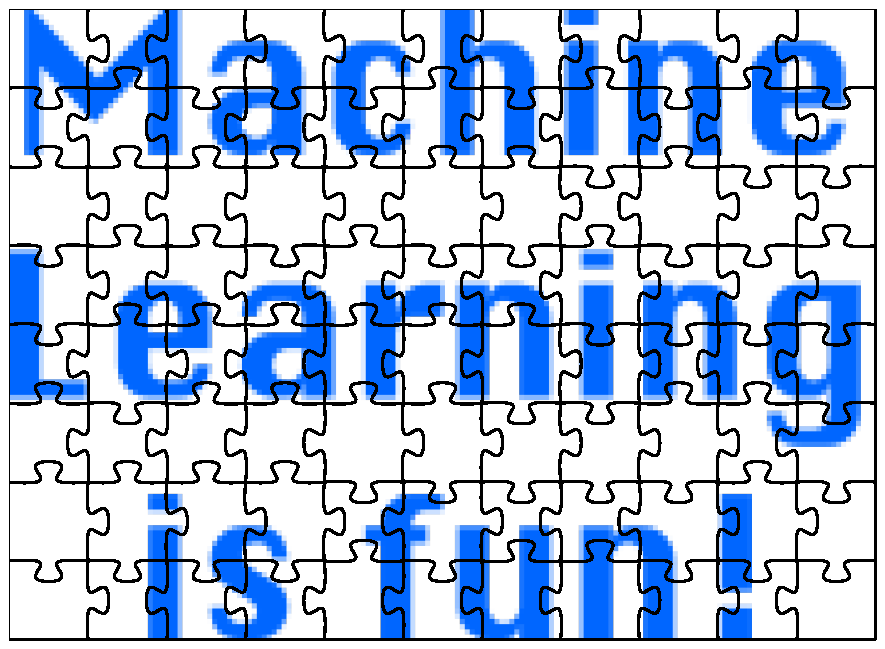
\includegraphics[width=11cm,height=8cm]{fig_ml_is_fun.png}};
		
		\def\xmax{10}
		\def\ymax{7}
		
		
		\foreach \x in {0,...,\xmax}{
			\foreach \y in {0,...,\ymax}{
				
				\ifnum\y=0
				\def\bottom{0}
				\else
				\pgfmathrandomitem{\bottom}{inout}%
				\fi
				
				\ifnum\x=\xmax
				\def\right{0}
				\else
				\pgfmathrandomitem{\right}{inout}%
				\fi
				
				\begin{scope}[xshift=\x cm, yshift=\y cm]
					\piece{\bottom}{\right}
				\end{scope}
			}
		}
		
		\draw (0,0) -- (0,\ymax+1) -- (\xmax+1,\ymax+1);
		
	\end{tikzpicture}
	
\end{document}